%!TEX root = cours.tex
\chapter{Tests et conditions}
\introduction{Ceci n'est pas un test !}
\section{Des outils pour comparer}

Ce sont les \textit{opérateurs de comparaison} :\\

{\small
\tabularstyled
\begin{tabular}{CCC}
	\rowcolor{lightgray}
	\rowcolor{UGLiOrange}{\boxfont\color{white} Opérateur} & {\boxfont\color{white} Signification} & {\boxfont\color{white} Remarques}                                                                     \\

	\mintinline{python}{<}                                       & strictement inférieur                 & Ordre usuel sur \mintinline{python}{int} et \mintinline{python}{float}, lexicographique sur \mintinline{python}{str}... \\

	\mintinline{python}{<=}                                      & inférieur ou égal                     & Idem                                                                                                  \\

	\mintinline{python}{>}                                       & strictement supérieur                 & Idem                                                                                                  \\

	\mintinline{python}{>=}                                      & supérieur ou égal                     & Idem                                                                                                  \\

	\mintinline{python}{==}                                      & égal                                  & \og avoir même valeur\fg\  \textit{Attention :} deux signes =                                         \\

	\mintinline{python}{!=}                                      & différent                             &                                                                                                       \\

	\mintinline{python}{is}                                      & identique                             & être le même objet                                                                                    \\

	\mintinline{python}{is not}                                  & non identique                         &                                                                                                       \\

	\mintinline{python}{in}                                      & appartient à                          & avec \mintinline{python}{str}, \mintinline{python}{list} et \mintinline{python}{dict}                                   \\

	\mintinline{python}{not in}                                  & n'appartient pas à                    & avec \mintinline{python}{str} et \mintinline{python}{list} et \mintinline{python}{dict}                                 \\
\end{tabular}
}\normalsize

\begin{pys}
	\begin{minted}{python}
>>> a = 2
>>> a == 2
>>> a == 3
>>> a == 2.0
>>> a is 2.0
>>> a != 100
>>> a > 2
>>> a >= 2
    \end{minted}
\end{pys}

\begin{pys}
	\begin{minted}{python}
>>> a = 'Alice'
>>> b = 'Bob'
>>> a < b
>>> 'e' in a
>>> 'e' in b
>>> liste = [1,10,100]
>>> 2 in liste
    \end{minted}
\end{pys}

Ces opérateurs permettent de réaliser des tests basiques. Pour des tests plus évolués on utilisera des \og mots de liaison \fg{} logiques.

\section{Les connecteurs logiques}

\begin{itemize}
	\item   \mintinline{python}{and} permet de vérifier que 2 conditions sont \textit{vérifiées simultanément}.
	\item   \mintinline{python}{or} permet de vérifier qu'\textit{au moins une} des deux conditions est vérifiée.
	\item   \mintinline{python}{not} est un opérateur de \textit{négation} très utile quand on veut par exemple vérifier qu'une condition est fausse.
\end{itemize}
Voici les tables de vérité des deux premiers connecteurs :
\tabularstyled{white}
\begin{center}
	\begin{tabular}{|c|c|c|}
		\hline
		\mintinline{python}{and} &\cellcolor{UGLiOrange}{\boxfont\color{white}True}       & \cellcolor{UGLiOrange}{\boxfont\color{white}False}       \\
		\hline
		\cellcolor{UGLiOrange}{\boxfont\color{white}True}      & \mintinline{python}{True}  & \mintinline{python}{False} \\
		\hline
		\cellcolor{UGLiOrange}{\boxfont\color{white}False}     & \mintinline{python}{False} & \mintinline{python}{False} \\
		\hline
	\end{tabular}\hspace{2em}
	\begin{tabular}{|c|c|c|}
		\hline
		\mintinline{python}{or} &\cellcolor{UGLiOrange}{\boxfont\color{white}True}       & \cellcolor{UGLiOrange}{\boxfont\color{white}False}       \\
		\hline
		\cellcolor{UGLiOrange}{\boxfont\color{white}True}      & \mintinline{python}{False}  & \mintinline{python}{True} \\
		\hline
		\cellcolor{UGLiOrange}{\boxfont\color{white}False}     & \mintinline{python}{True} & \mintinline{python}{True} \\
		\hline
	\end{tabular}
\end{center}
À ceci on peut ajouter que \mintinline{python}{not True} vaut \mintinline{python}{False} et vice-versa.

\begin{pys}
	\begin{minted}{python}
>>> True and False
>>> True or False
>>> not True
    \end{minted}
\end{pys}

\begin{pys}
	\begin{minted}{python}
>>> resultats = 12.8
>>> mention_bien = resultats >= 14 and resultats < 16
>>> print(mention_bien)
    \end{minted}
\end{pys}

\section{if, else et elif}
Voici le schéma de fonctionnement d'un test \mintinline{python}{if} :
\begin{center}
	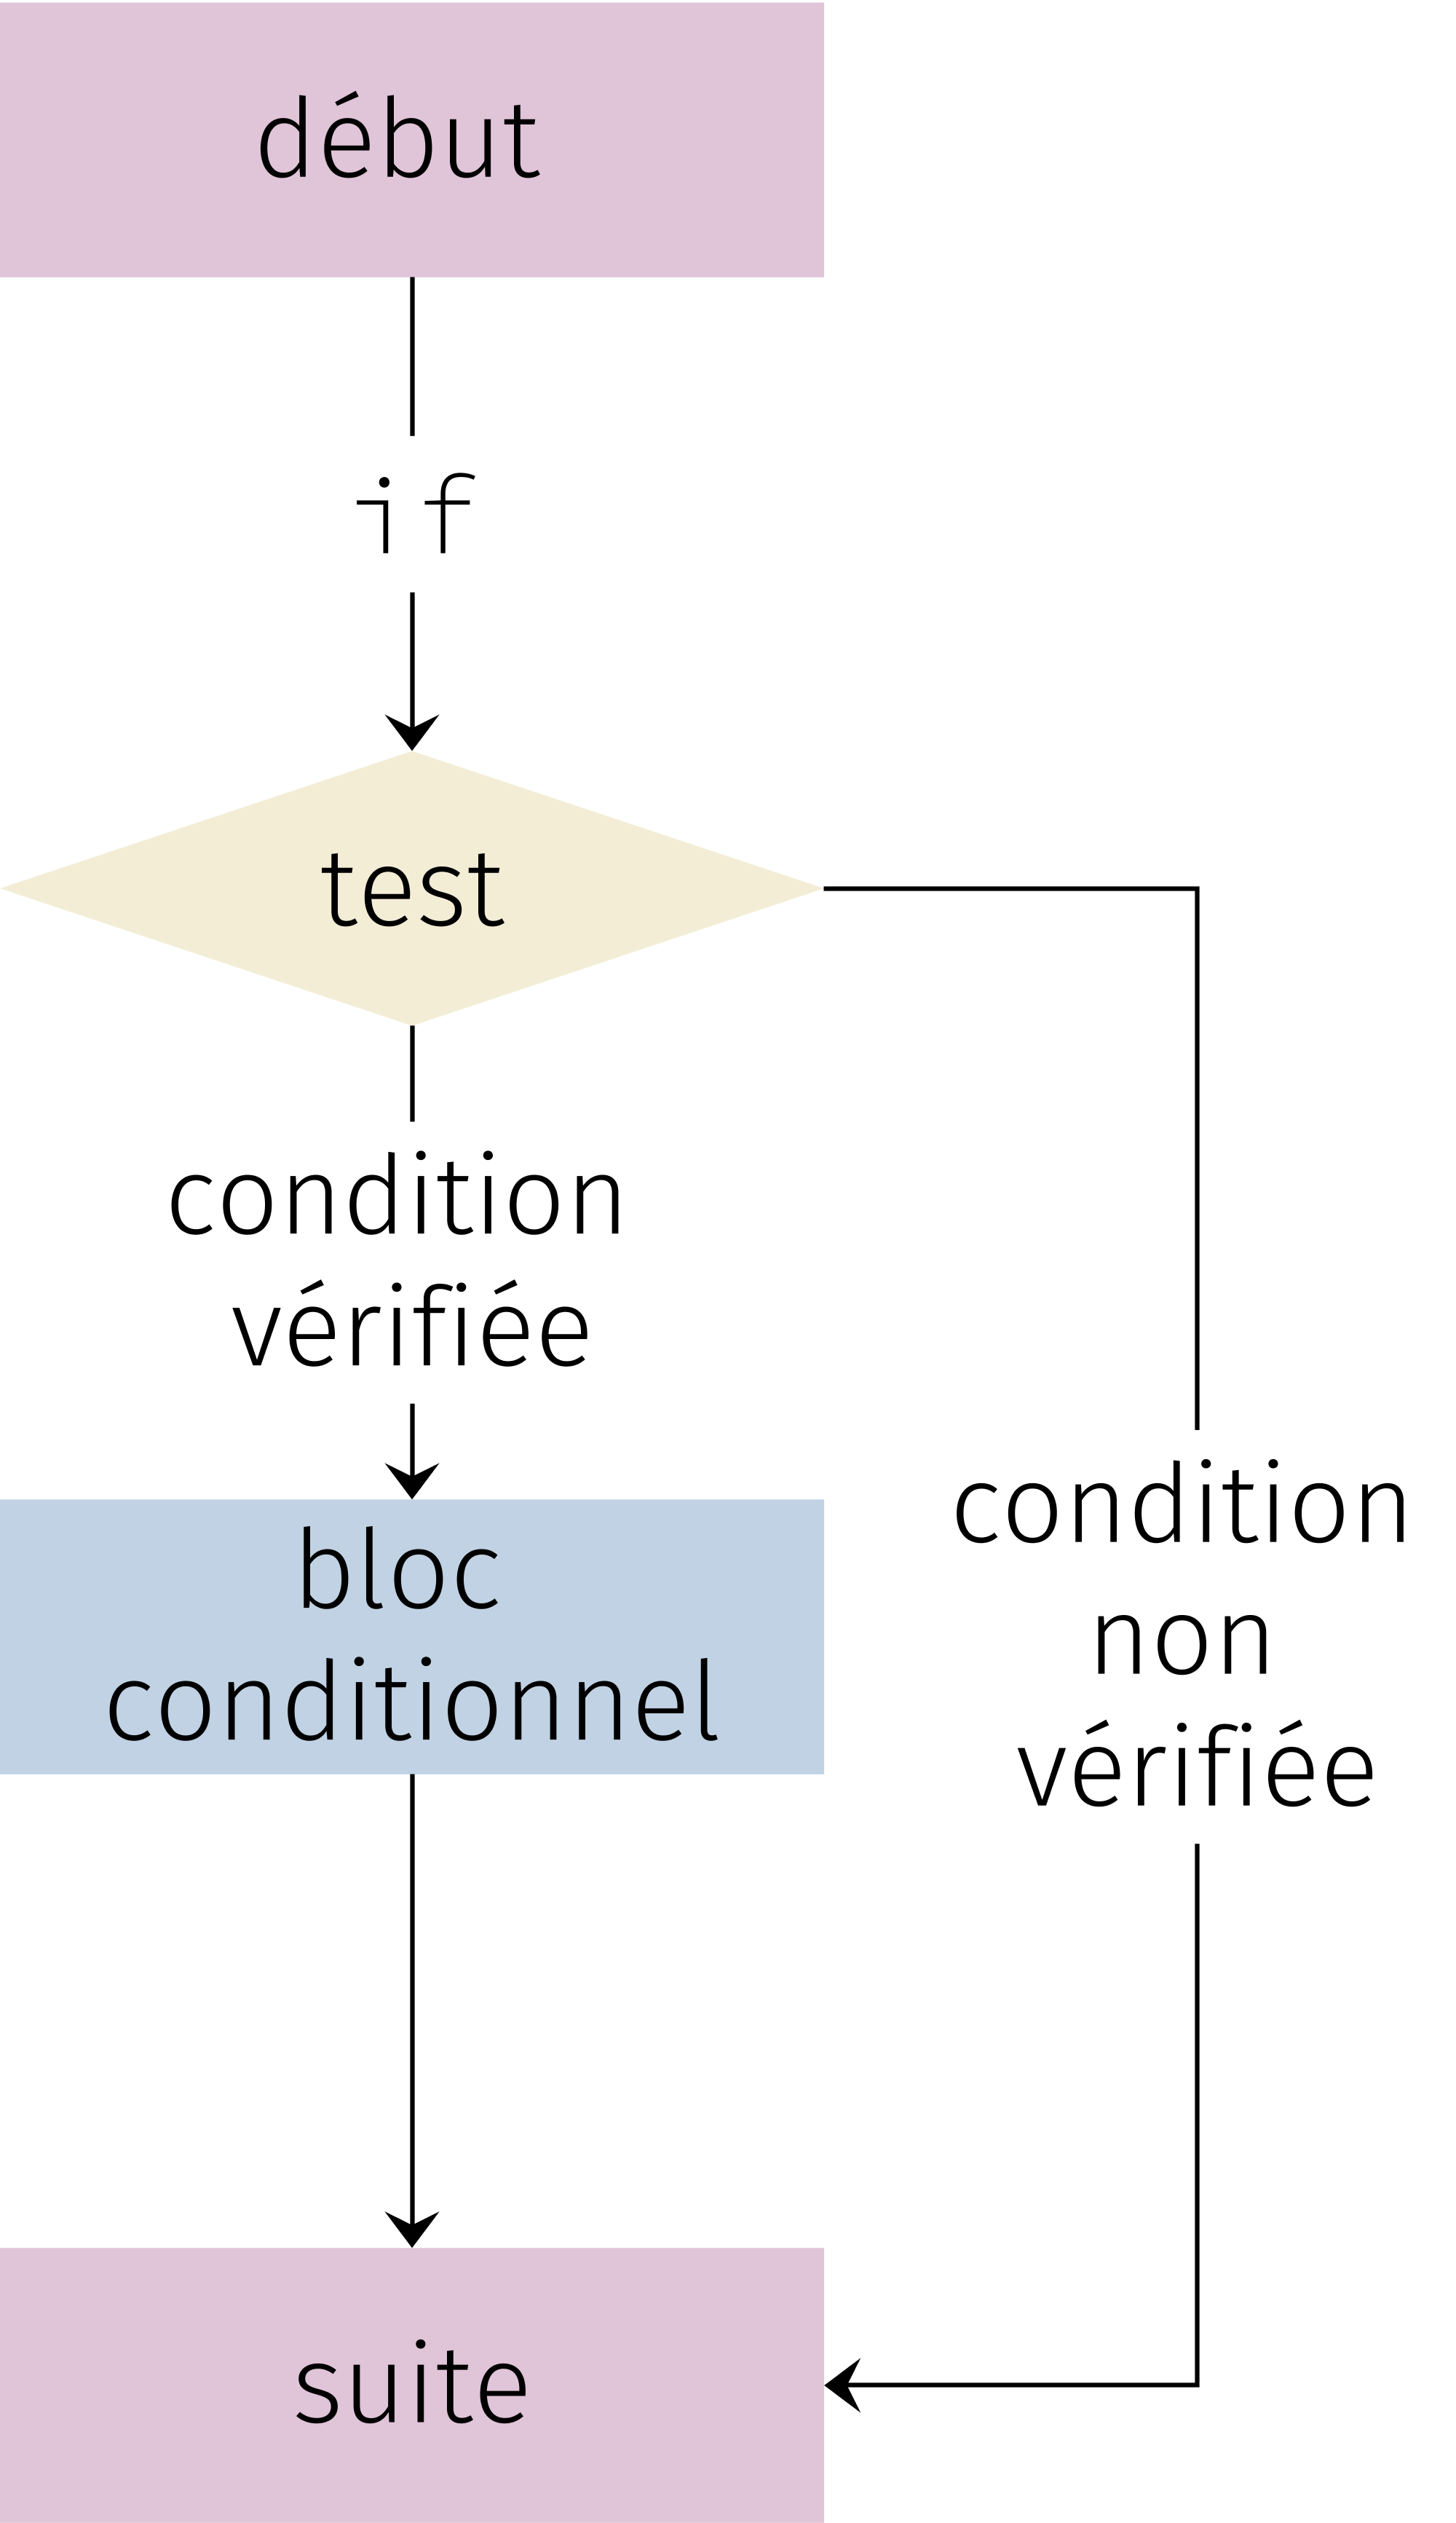
\includegraphics[height=8cm]{ch-conditions/img/if}
\end{center}

\textbf{Attention :} Un bloc conditionnel doit être \textit{tabulé} par rapport à la ligne précédente : il n'y a ni \mintinline{python}{DébutSi}  ni \mintinline{python}{FinSi}
en \textsc{Python}, ce sont les tabulations qui délimitent les blocs.

\begin{pyc}
	\begin{minted}{python}
phrase ='Je vous trouve très joli'
reponse = input('Etes vous une femme ?(O/N) : ')
if reponse == 'O':
    phrase += 'e'
phrase +='.'
print(phrase)
\end{minted}
\end{pyc}

Voici le schéma de fonctionnement d'un test \mintinline{python}{if...else} :
\begin{center}
	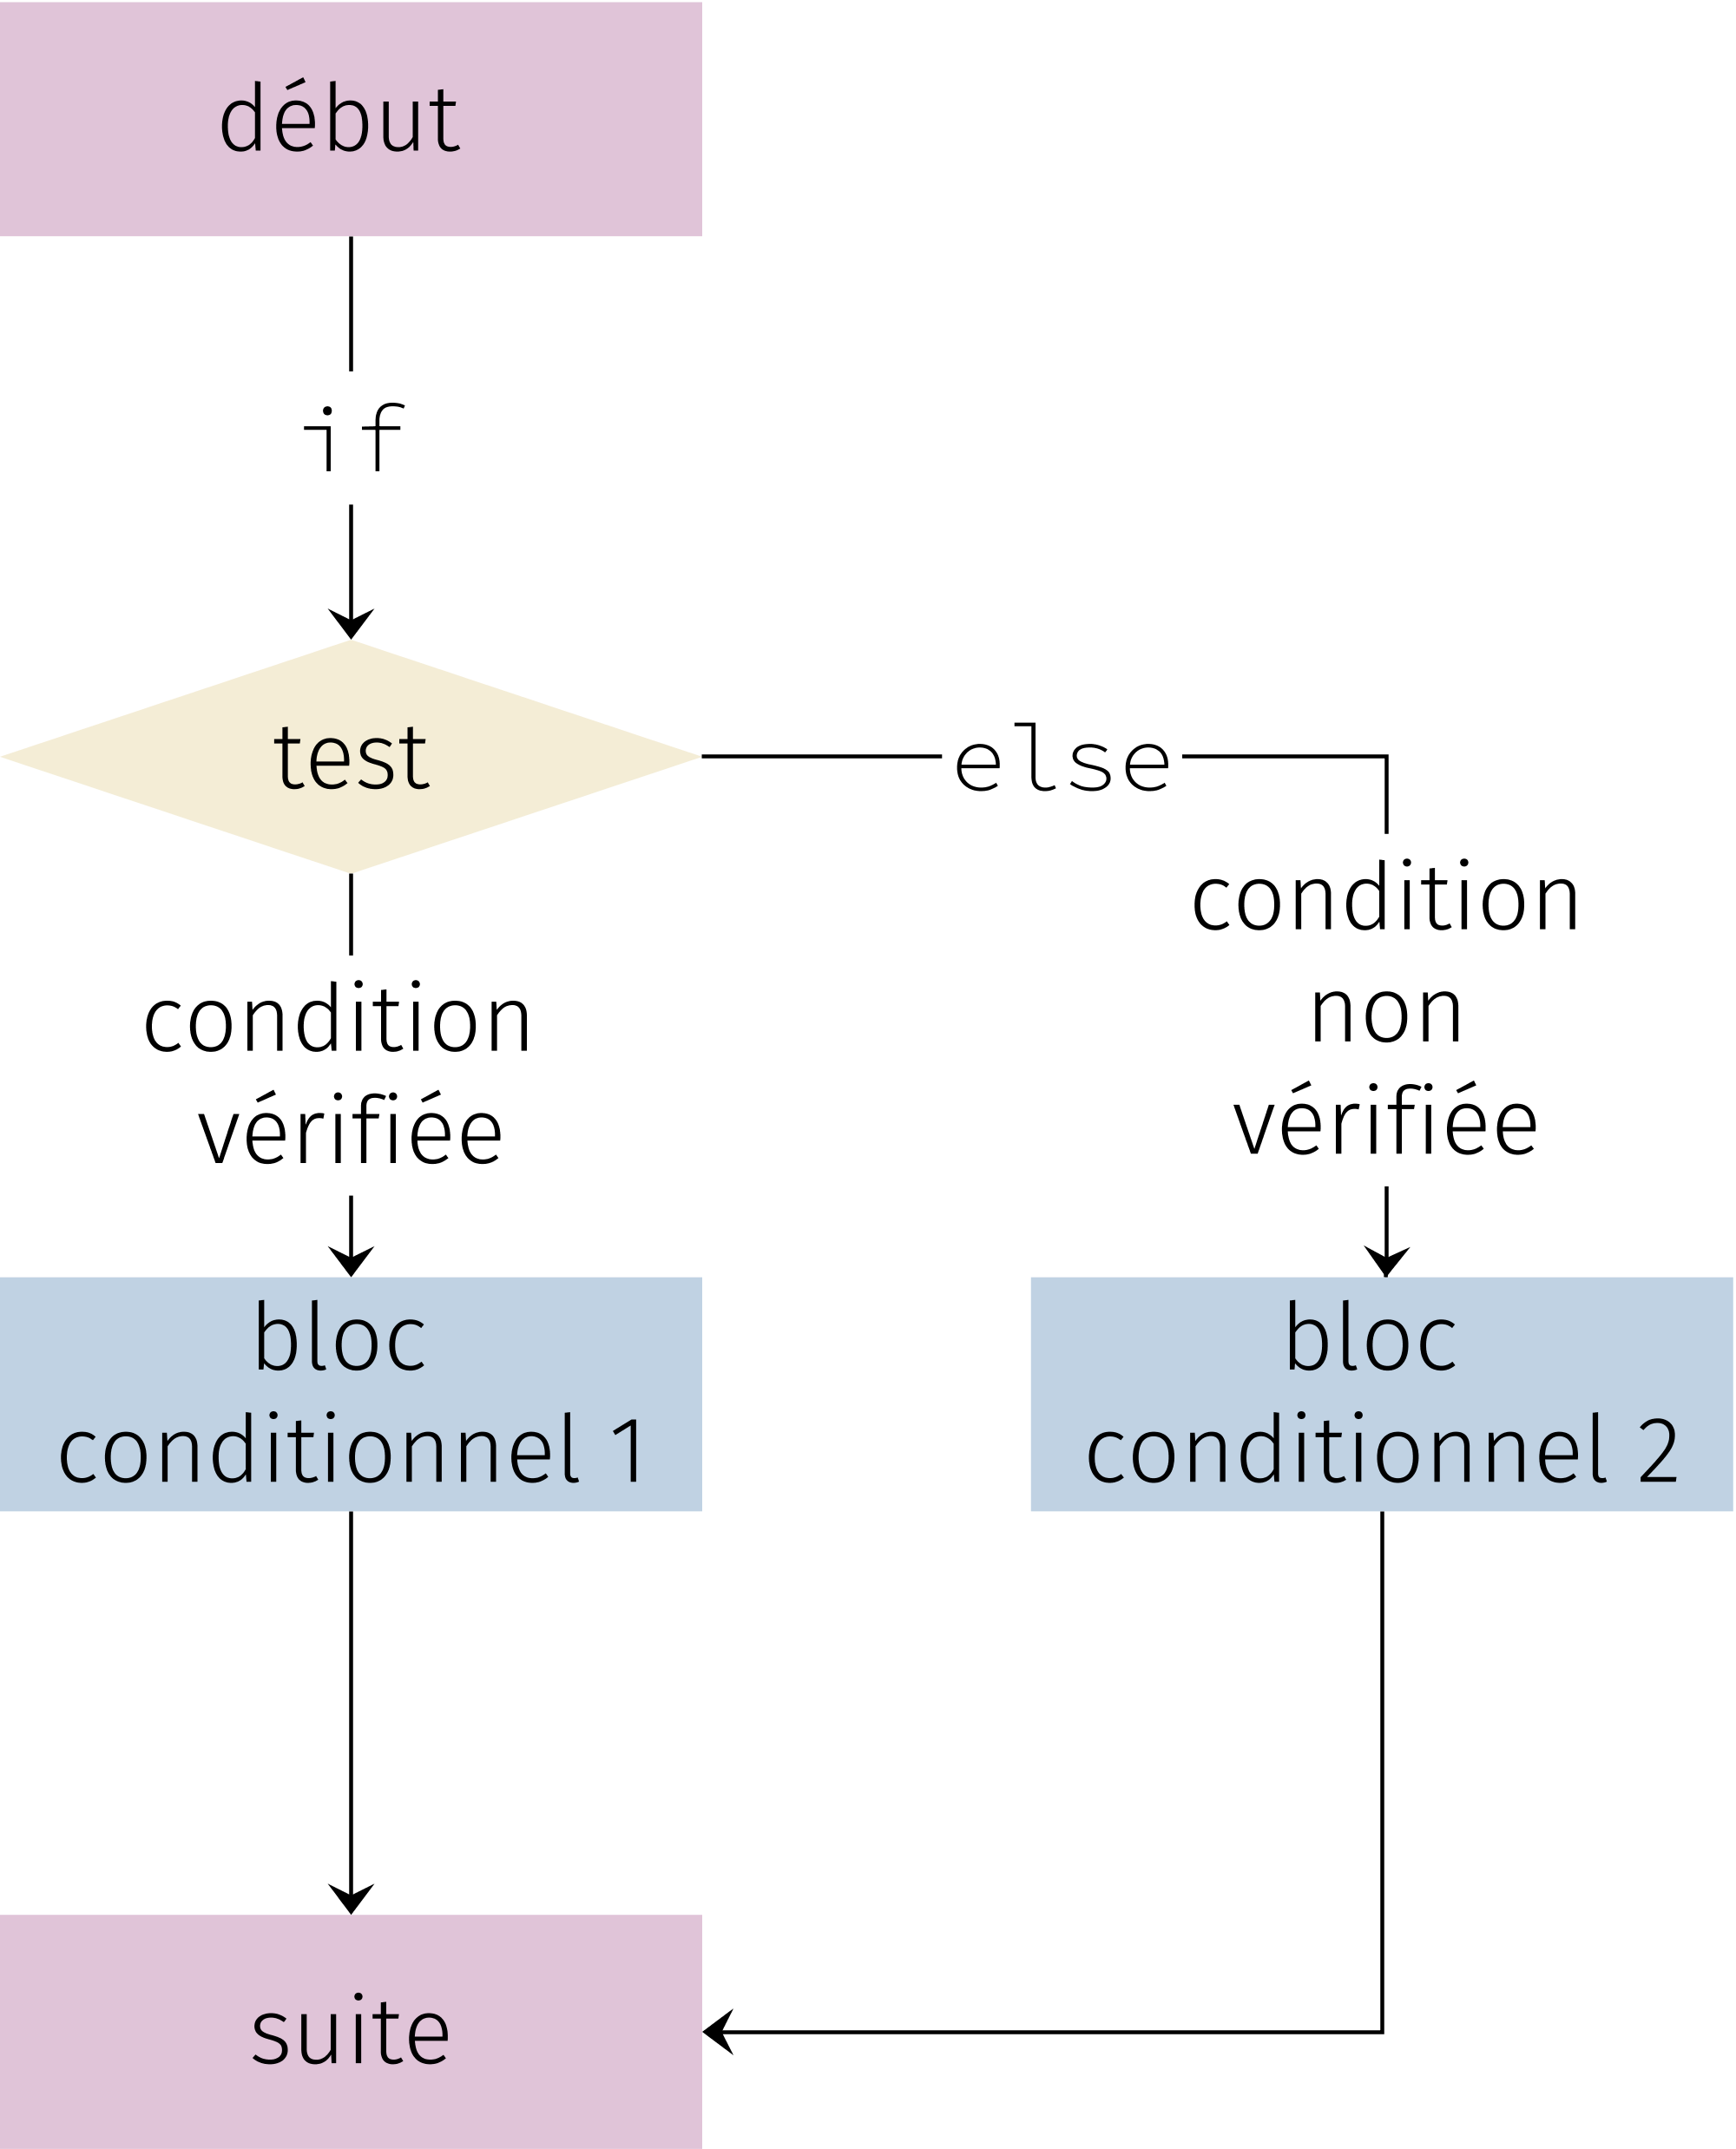
\includegraphics[height=8cm]{ch-conditions/img/ifelse}
\end{center}

\begin{pyc}
	\begin{minted}{python}
print('Bonjour')
age = int(input('Entrez votre age : '))
if age >= 18:
    print('Vous etes majeur')
else:
    print('Vous etes mineur.')
print('Au revoir.')
\end{minted}
\end{pyc}

Voici un exemple de fonctionnement d'un test \mintinline{python}{if...elif...} :
\begin{pyc}
	\begin{minted}{python}
print('Bonjour')
prenom = input('Entrez un prénom : ')
if prenom == 'Robert':
    print("Robert, c'est le prénom de mon grand-père.")
elif prenom == 'Raoul':
    print("Mon oncle s'appelle Raoul.")
elif prenom == 'Médor':
    print("Médor, comme mon chien !")
else:
    print("Connais pas")
print('Au revoir.')
\end{minted}
\end{pyc}
Et voici un schéma décrivant son fonctionnement :
\begin{center}
	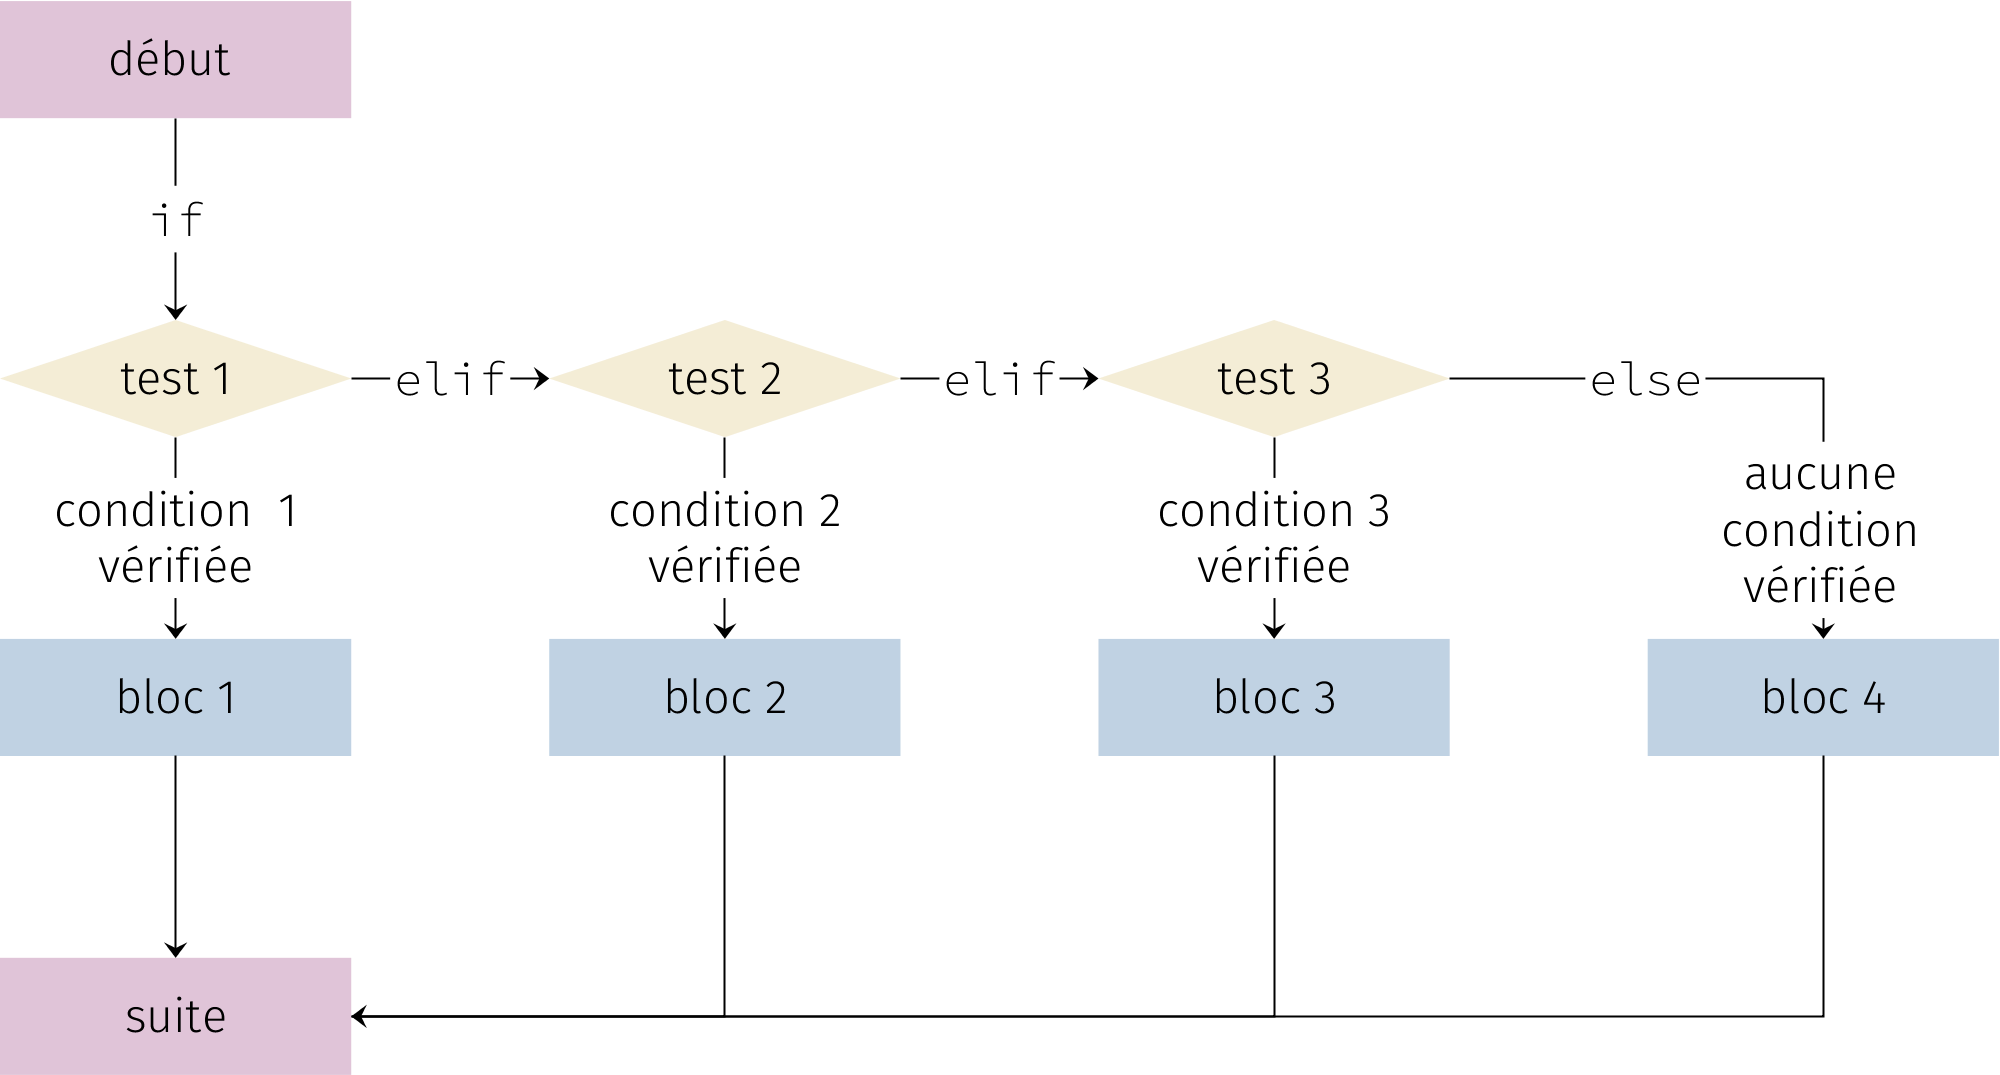
\includegraphics[width=\linewidth]{ch-conditions/img/ifelifelse}
\end{center}



On peut bien sûr inclure autant de \mintinline{python}{elif} que nécessaire.

\section{Exercices}

%----------------------------------------------------------------------
\begin{exercice}
	\'Ecrire un script qui demande son âge à l'utilisateur puis qui affiche \mintinline{python}{'Bravo pour votre longévité.'} si celui-ci est supérieur à 90.
\end{exercice}

\begin{exercice}[]
	\'Ecrire un script qui demande un nombre à l'utilisateur puis affiche si ce nombre est pair ou impair.
\end{exercice}
%----------------------------------------------------------------------
\begin{exercice}
	\'Ecrire un script qui demande l'âge d'un enfant à l'utilisateur puis qui l'informe ensuite de sa catégorie :
	\begin{itemize}
		\item   trop petit avant 6 ans;
		\item   poussin de 6 à 7 ans inclus;
		\item   pupille de 8 à 9 ans inclus;
		\item   minime de 10 à 11 ans inclus;
		\item   cadet à 12 ans et plus;
	\end{itemize}
\end{exercice}
%----------------------------------------------------------------------

\begin{exercice}
	\'Ecrire un script qui demande une note sur 20 à l'utilisateur puis vérifie qu'elle est bien comprise entre 0 et 20. Si c'est le cas rien ne se produit mais sinon le programme devra afficher un message tel que \mintinline{python}{'Note non valide.'}.
\end{exercice}

\begin{exercice}
	\'Ecrire un script qui demande un nombre à l'utilisateur puis affiche s'il est divisible par 5, par 7 par aucun ou par les deux de ces deux nombres.
\end{exercice}
%----------------------------------------------------------------------
\begin{exercice}
	En reprenant l'exercice du chapitre 1 sur les numéros de sécurité sociale, écrire un script qui demande à un utilisateur son numéro de sécurité sociale, puis qui vérifie si la clé est valide ou non.
\end{exercice}


%----------------------------------------------------------------------
\begin{exercice}
	\'Ecrire un script qui résout dans $\R$ l'équation du second degré $ax^2+bx+c=0$.\\
	On commencera par \mintinline{python}{from math import sqrt} pour utiliser la fonction \mintinline{python}{sqrt}, qui calcule la racine carrée d'un \mintinline{python}{float}.

	On rappelle que lorsqu'on considère une équation du type $ax^2+bx+c=0$
	\begin{itemize}
		\item   si $a=0$ ce n'est pas une équation de seconde degré;
		\item   sinon on calcule $\Delta = b^2-4ac$ et
		      \begin{itemize}
			      \item   Si $\Delta<0$ l'équation n'a pas de solutions dans $\R$;
			      \item   Si $\Delta=0$ l'équation admet pour unique solution $\dfrac{-b}{2a}$;
			      \item   Si $\Delta>0$ l'équation admet 2 solutions : $\dfrac{-b-\sqrt{\Delta}}{2a}$ et $\dfrac{-b+\sqrt{\Delta}}{2a}$.
		      \end{itemize}
	\end{itemize}
	Pour vérifier que le script fonctionne bien on pourra tester les équations suivantes :
	\begin{itemize}
		\item   $2x^2+x+7=0$ (pas de solution dans $\R$);
		\item   $9x^2-6x+1=0$ (une seule solution qui est $\dfrac{1}{3}$);
		\item   $x^2-3x+2$ (deux solutions qui sont 1 et 2).
	\end{itemize}
\end{exercice}

%----------------------------------------------------------------------
\begin{exercice}
	L'opérateur \mintinline{python}{nand} est défini de la manière suivante : si \mintinline{python}{A} et \mintinline{python}{B} sont deux booléens alors
	\begin{center}
		\mintinline{python}{A nand B} vaut \mintinline{python}{not (A and B)}
	\end{center}
	Construire la table de vérité de \mintinline{python}{nand} en complétant :
	\begin{center}
		\tabularstyled
		\begin{tabular}{|c|c|c|c|}
			\hline
			\rowcolor{UGLiOrange}{\boxfont\color{white} A} & {\boxfont\color{white} B} & {\boxfont\color{white} A and B} & {\boxfont\color{white} not (A and B)} \\
			\hline
			\mintinline{python}{False}                           & \mintinline{python}{False}      &                                 &                                       \\
			\hline
			\mintinline{python}{False}                           & \mintinline{python}{True}       &                                 &                                       \\
			\hline
			\mintinline{python}{True}                            & \mintinline{python}{False}      &                                 &                                       \\
			\hline
			\mintinline{python}{True}                            & \mintinline{python}{True}       &                                 &                                       \\
			\hline
		\end{tabular}
	\end{center}
\end{exercice}


